\documentclass[11pt]{article}
\usepackage[margin=0.9in]{geometry}
\usepackage{amsmath,amssymb}
\usepackage{booktabs}
\usepackage{graphicx}
\usepackage{fancyhdr}
\usepackage[hidelinks]{hyperref}

\graphicspath{{Figures/}}
\pagestyle{fancy}
\fancyhf{}
\lhead{STAT 546 \textbar{} HW5 implementation report \textbar{} Anurag Ramesh}
\rhead{30 October 2026}
\cfoot{\thepage}
\renewcommand{\headrulewidth}{0.4pt}
\setlength{\headheight}{14pt}
\setlength{\parindent}{0pt}
\setlength{\parskip}{6pt}

\begin{document}

All code is in \texttt{Scripts/}, one script per question. The general methods are in the root module
\path{High_Dimensional_Regression.py}. Each script saves its figures in \texttt{Figures/} and its numbers
in \texttt{Results/}. I used Python, with scikit-learn supplying the Lasso solver.

\section*{Q1. Learning the Gaussian graphical model}

I generated $n = 300$ independent observations from $N_{400}(0,\Theta^{-1})$, using the concentration
matrix exactly as given: diagonal 1, first off-diagonals 0.5, second off-diagonals 0.25, and zero elsewhere.
The zero mean is an assumption. The smallest eigenvalue of $\Theta$ is 0.25005, so it is positive definite.
I used a Cholesky factor $LL^T=\Theta$ and generated $x=L^{-T}z$, where $z\sim N_{400}(0,I)$.

I used nodewise Lasso (Meinshausen and B\"uhlmann, 2006). For a Gaussian distribution, an edge joins
variables $j$ and $k$ exactly when $\theta_{jk}\ne0$. After centring and scaling each column to mean
square 1, I regressed each standardized column $Z_j$ on all the others:
\[
\hat\gamma_j=\mathop{\arg\min}_{\gamma}
\left\{\frac{\|Z_j-Z_{-j}\gamma\|^2}{2n}+\lambda_G\|\gamma\|_1\right\},
\qquad \lambda_G=\sqrt{\frac{2\log p}{n}}=0.19986.
\]
This penalty was fixed without using the true graph. I included an edge when both regressions selected
the pair (the AND rule), treating coefficients below $10^{-8}$ in magnitude as zero. The OR rule includes
an edge if either regression selects it. Each undirected edge is counted once.

\begin{center}
\begin{tabular}{lrr}
\toprule
\textbf{Setting / result} & \textbf{AND} & \textbf{OR} \\
\midrule
Observations / variables / seed & \multicolumn{2}{c}{300 / 400 / 546} \\
True edges & \multicolumn{2}{c}{797} \\
Estimated edges & 551 & 650 \\
True positives / false positives / missed edges & 492 / 59 / 305 & 551 / 99 / 246 \\
Precision / recall & 0.893 / 0.617 & 0.848 / 0.691 \\
\bottomrule
\end{tabular}
\end{center}

The AND graph recovers much of the banded pattern, but misses 305 true edges. The OR rule recovers more
edges and also adds more false ones. Precision is the fraction of selected edges that are true; recall
is the fraction of the 797 true edges recovered. The figure shows the first 40 variables; the table
uses all 400.

\begin{center}
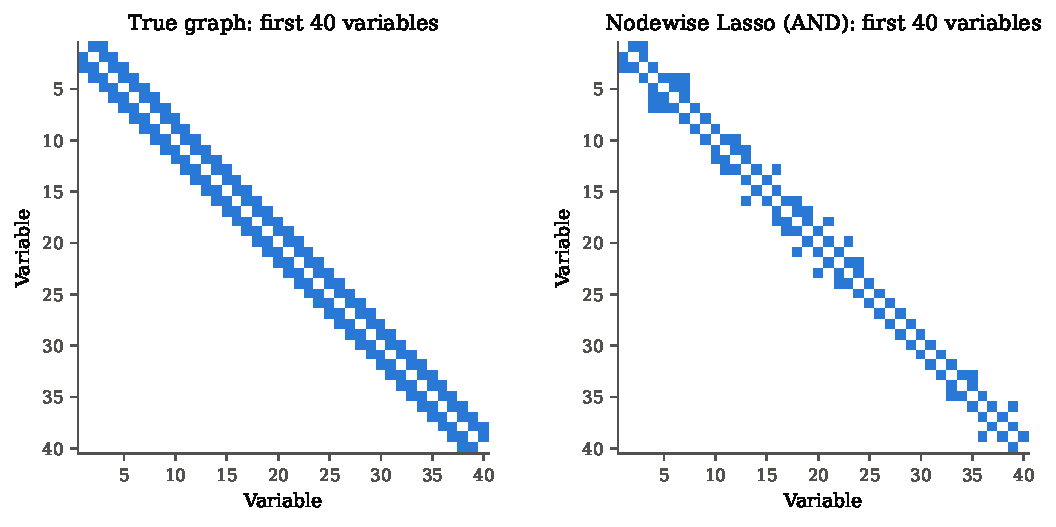
\includegraphics[width=0.72\textwidth]{q1_gaussian_graph.pdf}
\end{center}

\newpage
\section*{Q2. High-dimensional regression inference}

\subsection*{Data and fitting}

I used the same predictor matrix as in Q1 and generated
\[
y_i=1+2x_{i1}+2.5x_{i2}+3x_{i3}+3.5x_{i4}+4x_{i5}+\epsilon_i.
\]
The remaining 395 slopes are zero. The assignment does not specify the errors; I used independent
$\epsilon_i\sim N(0,1)$, independent of the predictors, with seed 547.

I used desparsified Lasso (van de Geer et al., 2014). Let $Z_{ij}=(x_{ij}-\bar x_j)/s_j$, with
$s_j^2=n^{-1}\sum_i(x_{ij}-\bar x_j)^2$, and let $y_c=y-\bar y$. I first fitted
\[
\hat a=\mathop{\arg\min}_a
\left\{\frac{\|y_c-Za\|^2}{2n}+\lambda_Y\|a\|_1\right\}.
\]
Five-fold cross-validation chose $\lambda_Y$ by minimum prediction error over 40 logarithmically spaced
values from 0.01 to 0.5. Each fold fitted its own centring and scaling on the training observations.
The intercept was not penalized.

\subsection*{Bias correction and uncertainty}

I used a separate nodewise penalty $\lambda_N$ for inference. It was selected by five-fold
cross-validation, averaging prediction error over all 400 nodewise regressions, from 20 logarithmically
spaced values from 0.01 to 0.3. This choice uses only the predictors. Graph selection in Q1 and the
approximate inverse needed here have different purposes, so their penalties need not agree.

For each nodewise fit, let $r_j=Z_j-Z_{-j}\hat\gamma_j$ and define
\[
\hat\tau_j^2=\frac{r_j^Tr_j}{n}+\lambda_N\|\hat\gamma_j\|_1,
\qquad
M_{jj}=\frac{1}{\hat\tau_j^2},\quad
M_{j,-j}=-\frac{\hat\gamma_j^T}{\hat\tau_j^2},\quad Q=ZM^T.
\]
I kept $M$ as this rowwise approximate inverse of the sample correlation matrix. With
$e=y_c-Z\hat a$, the corrected coefficients and their standard errors in the original units are
\[
\hat b_j=\frac{\hat a_j+Q_j^Te/n}{s_j},
\qquad
\widehat{\mathrm{se}}_j=\frac{\hat\sigma\|Q_j\|}{ns_j},
\qquad
\hat\sigma^2=\frac{e^Te}{n-\hat s-1},
\]
where $\hat s$ is the number of nonzero slopes in the initial Lasso. The residual degrees-of-freedom
correction estimates the noise variance; it is not an exact unbiased estimate after selection.

I formed pointwise 95\% intervals $\hat b_j\pm1.96\widehat{\mathrm{se}}_j$ and two-sided normal p-values
for $H_{0j}:\beta_j=0$. For testing all 400 slopes, I used
$p_{j,\mathrm{adj}}=\min(1,400p_j)$ and rejected at 0.05. The intervals are marginal, not simultaneous.
This inference relies on a high-dimensional normal approximation and sufficiently small remaining
regularization bias; it is not an exact finite-sample guarantee.

\newpage
\subsection*{Results}

\begin{center}
\begin{tabular}{p{0.52\textwidth}p{0.38\textwidth}}
\toprule
\textbf{Setting / result} & \textbf{Value} \\
\midrule
Observations / variables / design seed & 300 / 400 / 546 \\
Cross-validation folds / shuffle seed & 5 / 546 \\
Selected $\lambda_Y$ / selected $\lambda_N$ & 0.08219 / 0.08569 \\
Initial nonzero slopes / estimated error SD & 50 / 1.078 \\
Solver tolerance / maximum iterations & $10^{-8}$ / 10,000 \\
\textbf{Bonferroni-significant variables} & \textbf{1, 2, 3, 4, 5} \\
\bottomrule
\end{tabular}
\end{center}

The five nonzero coefficients are shown below. Very small p-values are given as bounds; a numerical
underflow to zero does not mean that the mathematical p-value is zero.

\begin{center}
\begin{tabular}{rrrrlr}
\toprule
\textbf{Variable} & \textbf{True} & \textbf{Estimate} & \textbf{SE} & \textbf{95\% interval} & $\boldsymbol{p_{\mathrm{adj}}}$ \\
\midrule
1 & 2.0 & 1.748 & 0.059 & $[1.633,\ 1.863]$ & $<10^{-190}$ \\
2 & 2.5 & 2.240 & 0.057 & $[2.129,\ 2.351]$ & $<10^{-190}$ \\
3 & 3.0 & 2.791 & 0.056 & $[2.681,\ 2.901]$ & $<10^{-190}$ \\
4 & 3.5 & 3.281 & 0.050 & $[3.184,\ 3.378]$ & $<10^{-190}$ \\
5 & 4.0 & 3.818 & 0.052 & $[3.716,\ 3.919]$ & $<10^{-190}$ \\
\bottomrule
\end{tabular}
\end{center}

The adjusted tests identify all five nonzero slopes and no null slopes. Without adjustment, 12 of the
395 null slopes are significant at 0.05. The intercept estimate
$\hat b_0=\bar y-\bar x^T\hat b$ is 0.970, compared with the generating value 1.

\textbf{Interval check:} 383 of the 395 null intervals contain zero, but none of the five nonzero
coefficients lies in its interval. Their estimates are 0.182--0.260 below the true values. The bias
correction leaves substantial shrinkage in this correlated design, so the nominal 95\% intervals are
not reliable for these five coefficients in this run. The overall count, 383 out of 400, would hide
that failure. These counts describe one simulated dataset, not repeated-simulation coverage.

\begin{center}
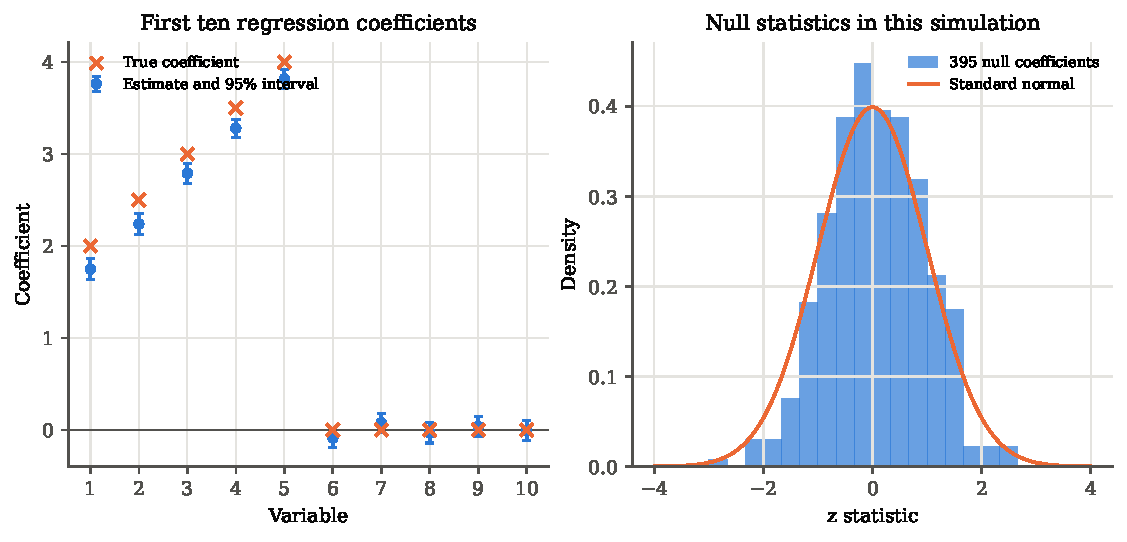
\includegraphics[width=0.88\textwidth]{q2_desparsified_lasso.pdf}
\end{center}

\newpage
\section*{Saved results}

The saved \texttt{q2.json} contains estimates, standard errors, intervals and raw and adjusted p-values
for every slope. The simulated predictors and concentration matrix are in \texttt{q1\_data.npz}; the
response, true slopes and errors are in \texttt{q2\_data.npz}.

\section*{References}

STAT 546, Fall 2026. Homework 5, Questions 1--2. The concentration matrix, regression coefficients and
requested methods are taken from the assignment.

N. Meinshausen and P. B\"uhlmann (2006). High-dimensional graphs and variable selection with the Lasso.
\emph{The Annals of Statistics}, 34(3), 1436--1462.
DOI: \href{https://doi.org/10.1214/009053606000000281}{10.1214/009053606000000281}.

S. van de Geer, P. B\"uhlmann, Y. Ritov and R. Dezeure (2014). On asymptotically optimal confidence
regions and tests for high-dimensional models. \emph{The Annals of Statistics}, 42(3), 1166--1202.
DOI: \href{https://doi.org/10.1214/14-AOS1221}{10.1214/14-AOS1221}.

\end{document}
